\chapter{Inferring the location of RTT changes}
\label{sec:infer}
\section*{Abstract}

\section{Perform measurement-based TE without direct measurements}
Locating the cause of RTT changes is an intriguing research topic in its own right.
Meanwhile, it is as well beneficial for measurement-based TE when measurements toward certain destination prefixes are not available.

\subsection{Lack of direction measurements}
\marginpar{How the RTT toward a destination prefix is measured?}
As explained in Section~\ref{sec:intro}, in order to measure the path performance toward a destination prefix, we need to, in first place, identify some hosts in that prefix that can be measured, or respond to our measurements.
One possible approach identifying them is to look for hosts listening on some common TCP ports, e.g. 80, 443 etc., in the traffic exchanged with that destination prefix or through port scanning.
Then RTT toward the destination prefix is represented by the measurements toward identified hosts~\footnote{Several ways exists to actively measure the RTT through TCP. Some methods with few footprint and low measurement are employed in port scanning~\cite{nmap}, like SYN (also known as half open) or FIN stealth.}.

\marginpar{Lack of direct measurement toward certain destination prefixes.}
However, not all selected destination prefixes have such hosts with open ports, and
consequently leaves measurement-based TE without measurements~\footnote{selected prefixes: destination prefixes with important volume thus selected for TE, more detail in Section~\ref{sec:pref_selec}.}.
Take client SA appeared in Section~\ref{sec:pref_selec} as an example, on average 15\% of its outbound traffic involving $\sim 330$ destination prefixes are without measurements.
More than 70\% of the `un-measured' traffic flows toward prefixes owned by mobile operators during peak hours.
In the foreseeable future, the proportion of such traffic would be even bigger, given the overall tendency of increasing usage on mobile devices.
At this point, we face with the problem of \textit{how to perform measurement-based TE without direct measurement toward the destination}. 

\subsection{Prefix Grouping as a countermeasure}
\marginpar{How about group `un-measurable' prefixes' with `measurable' ones?}
One possible approximation is to group `un-measurable' prefixes with those have measurements based on topological/geographical locality, for example those belonging to same AS or city. With that, measurements toward certain destination prefix represent multiple prefixes in the locality. And TE operations are uniformly performed for groups of prefixes.
The problem with the approach is two-fold. 

\marginpar{geographical locality}
First, locality is not necessary a good enough heuristics for shared fate in RTT performance. 
Assuming geographical locality, it at most provides a rough estimation on the baseline RTT in reaching a destination prefix, not regarding issues with the IP geolocation precision~\cite{Poese2011}. Plus, it does not necessary indicate similarity in paths, nor offer enough distinction on instant transmission performance if the actual paths employed are different for destinations prefixes in the group.

\marginpar{topological locality}
Assuming topological locality, say AS-level, is more relevant, but still not good enough.
As it has been pointed out, AS is not an atomic point~\cite{Muhlbauer2006}. Sub-AS structures can lead to difference in path chosen by others ASes in reaching its different prefixes. A recent study offers a close look on the heterogeneity of sub-AS routing behavior~\cite{Lee2016}. Finally, such approximation is helpless when the entire AS is not `measurable'.

\marginpar{Can the measurable speak for the rest?}
Second, in order to prove the effectiveness of such heuristics, one needs eventually measurements and the results could hence be biased toward/over-fitted for the part of Internet with measurements. Assuming the same for the rest without measurement data would be unconvincing.

\subsection{How RTT change cause inference can help?}
\marginpar{Treat the cause, not the symptom.}
Still, existing measurements, though toward destination other than the ones lack of them, can be taken advantage of. The idea is instead of finding replacement measurements for `un-measurable' prefixes, we can try identifying directly the causes for important RTT changes. As articulated in Section~\ref{sec:cpt_rtt}, changes in RTT measurements is the trigger for TE and is what we actually care about. If the identified cause for a RTT change, can be an AS or an inter-AS link, sit on the path toward the destination prefixes without measurements, we can reasonably assume that those `un-measurable' prefixes shall undergo similar RTT changes as well. Then further TE operations can be as well trigger for the `un-measurable' prefixes.

\marginpar{Intuitive on cause inference.}
The idea was initially inspired by the case study in Section~\ref{sec:ripe_case_study} on shared RTT changes by multiple RTT time series from different ASes. 
We realized that certain RTT changes can potentially have a big influence range.
Optimize the routing against the cause of such changes would be a more fundamental and effective approach to TE than handling each individual prefixes, henceforth RTT change cause inference.

Meantime, the case study implies that the cause for such shared RTT changes could lie in the common part of these impacted paths.
If given measurements on a single path that undergo RTT changes, it is impossible to tell which part of the path causes the changes. However, if multiple paths with common parts and divergent parts are measured and are impacted simultaneously by an RTT change, it is then possible to narrow down the potential cause to the common part of the path.

\section{Relationship to network delay tomography}

\subsection{Similarity in assumption and inference logic}
It is not difficult to spot that RTT change cause inference is somewhat similar to the quest of network delay tomography~\cite{Coates2002}, i.e. to infer the internal link delay characteristics using end-to-end measurements. The similarity not only lies in the formulation of the problem, but as well as in the assumptions and general idea of inference.

Many tomography works assume that measurements toward difference destinations experience similar delay on the shared links. As a matter of fact, these works either use multicast~\cite{LoPresti2002} or closely time spaced unicast measurements\cite{Shih2003,Tsang2003} to ensure this assumption. In our case, this intuitive assumption can be naturally extended: multiple RTT measurements shall undergo a same RTT change if caused by the common part on their paths.

The above assumption serves for inference. In delay tomography, since the common links contribute equally to end-to-end delay measurements, then the difference in end-to-end measurements can only come from the divergent part of the path. With carefully designed measurement sets, it is then possible to infer for each internal link its delay properties~\cite{Lawrence2006}.
The basic inference logic for RTT change cause inference follows the same spirit, yet in slightly different form. That is, if multiple end-to-end measurements with common and divergent part in their paths experience at the same time a significant RTT change, then the cause for this change probably comes from the common part.

\subsection{Difference in output}
Despite the similarity between the two problems, the fundamental outcome wanted at the end of inference differs.
In delay tomography, one wishes to reconstruct the the probability distribution of delay on internal links, where the likelihood of each end-to-end delay measurements is parameterized by a convolution of internal links' delay distribution, from source to destination.
The parameters for internal link delay distribution can then be solved through maximum likelihood estimation of the end-to-end path delay distributions given the end-to-end measurements.
For that purpose, a series of methods are developed either to accelerate the maximum-likelihood estimation of delay distribution~\cite{Liang2003, Tsang2003}, or to capture the time-varying nature of link delays~\cite{Shih2003,Coates2002a,Tsang2003}.
If we were to apply the same approach to our RTT measurements after changepoint detection (Section~\ref{sec:cpt_rtt}), we might arrive at a probability distribution on the likelihood of a link causing significant RTT change over the period of measurements. However, it doesn't tell at what exact moment the link caused a significant RTT change.

\subsection{Methodological compatibility}
\marginpar{Can we employ delay tomography methods for RTT change cause inference?}
Further, one might wonder whether it is possible to apply delay tomography methods directly to Internet RTT measurements over a relatively short time range. And then detect whether the delay distribution experiences obvious change over time, or exhibit multimodality for certain links.

This approach is however not the most appropriate for various reasons. First, the assumption of
same delay contribution from same link to different end-to-end measurements no longer holds for Internet RTT measurements for TE uses. It is because the timing of different measurements are not strictly synchronized. Rather, random factors are deliberately added to each individual measurement in building the real system to avoid creating periodic peaks of measurement traffic that might introduce interference among each other and hence harm measurement reliability. Moreover,  RIPE Atlas measurements (Section~\ref{sec:ripe_atlas}) wildly employed in this work do not guarantee strict synchronization among different measurements.
Those measurements are individually performed by probes loosely coordinated. The timing depends basically on the moment when each probe starts for the first time.
Second, delay tomography introduces potentially a scalability issue for Internet measurements, as it is first conceived for intradomain uses and are in most cases validated solely on simulated networks way much smaller than the actually part of the Internet over which the traffic of a typical content/hosting/service provider could span.

\section{RTT change cause inference}
\label{sec:inference}
In this section, we describe the inputs and output of the RTT change cause inference functionality, as well as its internal buildings blocks. The assumptions to initiate the inference are presented in a more formal way, along with..(complete this part later)
\subsection{The big picture}

\begin{figure}[!htb]
\centering
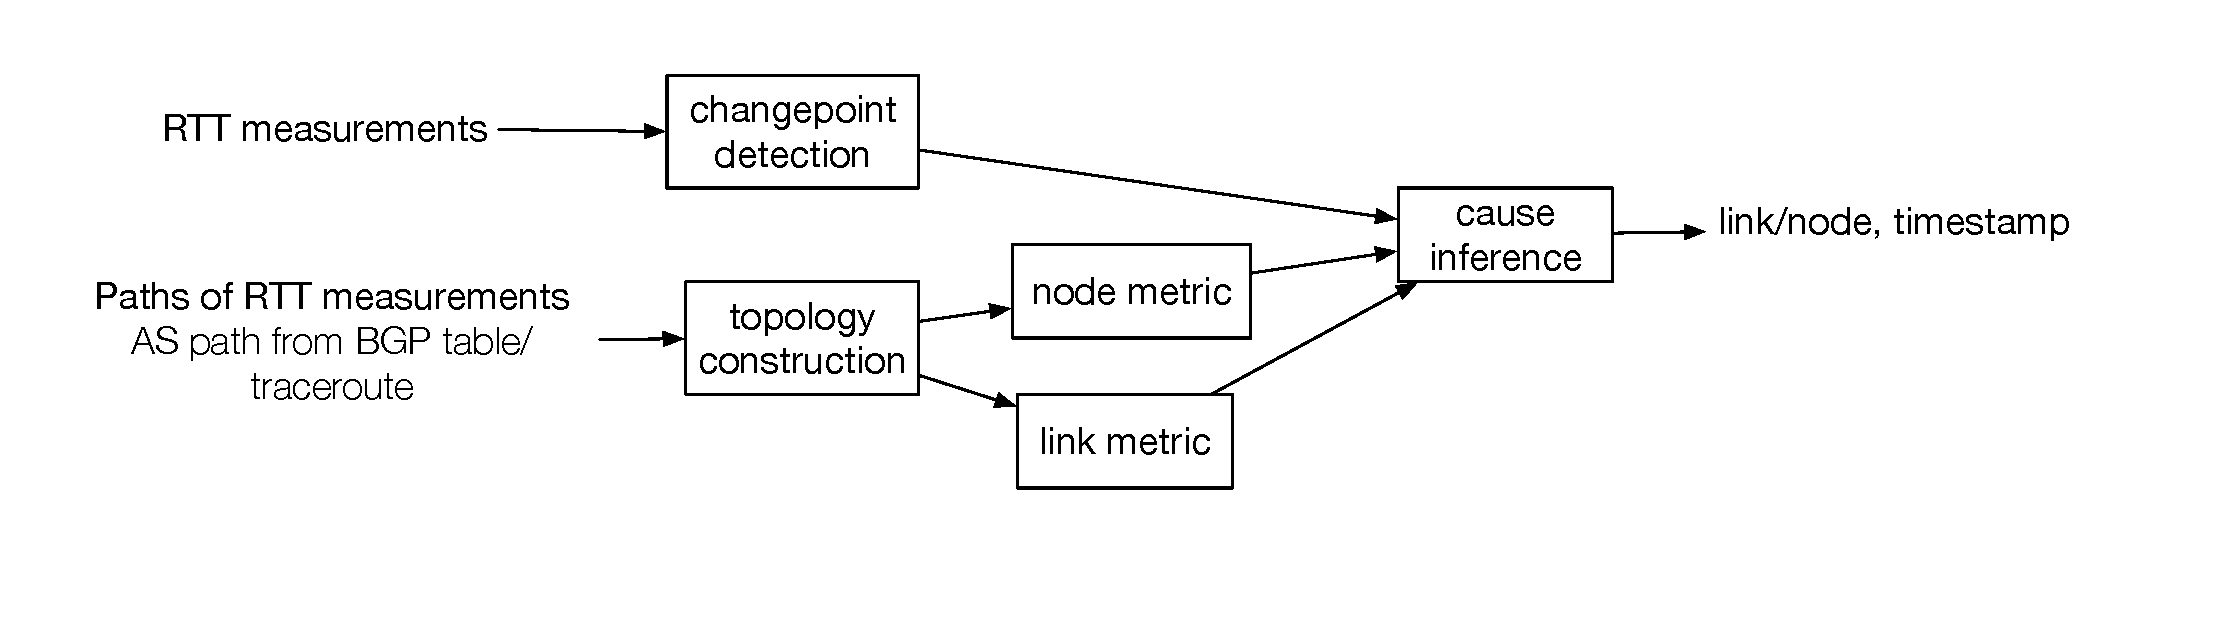
\includegraphics[width=1.5\textwidth]{gfx/chap5/sys_design.pdf}
\caption{Building blocks of RTT change cause inference.}
\label{fig:chap5_sys_design}
\end{figure}

\marginpar{input and output}
With RTT change cause inference, we are interested in identifying the part of the Internet, as precise as possible, that is responsible for RTT changes detected. What we have as input on client TE platforms are 1) RTT measurements from multiple sources to multiple destinations for TE uses; 2) underlying AS path for these RTT measurements~\footnote{With real TE system, the sources are client platforms and destinations are destination prefixes clients send traffic to. The source of measurements could be multiple if we merge measurements from multiple client platforms or the client has multiple sites with different provider options.}. 

\marginpar{Justify the usage of RIPE Atlas measurements.}
In this work, we continue to use the same data collected for RTT change detection in Section~\ref{sec:cpt_rtt} as replacement for client data for the sake of transparency and repoducibility. The major difference with the data available on TE client platform is that, with RIPE Atlas, the underlying path is learnt through traceroute instead of from BGP table~\footnote{It is though as well possible to learn paths of RTT measurements via RIPE RIS~\cite{ris}and Routeviews~\cite{routeviews}, the limited coverage of those BGP vintage points doesn't necessary reflect how each hosting AS of Atlas probes route the traffic.}. 
Such difference calls for additional pre-processing, such as IP-to-AS translation, IXP detection etc. It however should not have impact on the inference logic. On the other hand, given the worldwide distribution of RIPE Atlas probes and divers destinations they probe, the inference result from RIPE Atlas can complement that from client platform measurements, by offering a larger coverage of the Internet, hence bigger possibility of identifying cause of changes having impact on `un-measurable' destination prefixes.

\marginpar{building blocks}
Fig.~\ref{fig:chap5_sys_design} depicts the logical building blocks required for RTT change cause inference. Changepoint detection (Section~\ref{sec:cpt_rtt}) transforms the RTT timeseries into sequences of 0 and 1. Moments of 1 indicate the occurrences of significant RTT change.
Topology construction builds a graph for hops and links traversed by RTT measurements.
This topology graph is an intermediate step for the conception of inference metric for nodes and links present in the graph. Intuitively, we can tell whether a node/link is the cause for RTT change, depends on the measurements that traverse it and yet are topologically disjoint except the node/link in question. Identifying such measurement sets for each node/link requires topology knowledge and is key for building numerical inference metrics. Moreover, the topology graph serves as well in industrializing the location of RTT changes. 
The changepoint detection results instantiate the inference metrics.
The later is then consumed by the inference logic, which outputs the links and nodes that are responsible for RTT changes at a specific moments.

\subsection{Spatial and temporal granularity of inference}
\subsubsection{Spatial granularity}
Spatial granularity defines the finest element to which an RTT change cause can be attributed to.
It basically depends on the the granularity of the path and topology graph. We settled on AS-level granularity for following reasons, though it is possible to reconstruct IP-level or router-level topology\cite{Donnet2007} from traceroute measurements from RIPE Atlas.

First, to be compatible with data available on client TE platform. Theoretically, nothing prevents the client TE platform from performing periodic traceroute measurements for all the selected destination prefixes. However, in practice, path information is mainly learnt from BGP table and traceroute is only performed on demand. The main reason is that traceroute measurement is much  more costly than RTT measurements in CPU, I/O and storage resources. Plus, IP-level path information is plainly not needed in making interdomain level decisions most of the time.

Second, under intradomain TE frameworks, sub-AS level networking issues can mainly be avoided at AS level. Imagine there is a \acf{PoP} -level issue impacting some of the measurable and `un-measurable' prefixes. For measured prefixes, we can tell whether any of its available paths are impacted by measurements. While, for `un-measurable' prefixes, there is just no way to tell whether its paths traverse that problematic PoP or not. The safest would be to avoid that AS if possible.

%Third, constructing sub-AS level topology is not trivial.

\subsubsection{Temporal granularity}


\subsection{Assumptions}

\subsection{Inference metric and logic}
\subsubsection{Node}
\subsection{Link}

\section{Case studies}
